% Copyright (C) 2019 Esote.
% Permission is granted to copy, distribute and/or modify this document
% under the terms of the GNU Free Documentation License, Version 1.3
% or any later version published by the Free Software Foundation;
% with no Invariant Sections, no Front-Cover Texts, and no Back-Cover Texts.
% A copy of the license is included in the section entitled "GNU
% Free Documentation License".

% Images are copyright their respective authors.

\documentclass{beamer}
\usepackage{hyperref}

\newcommand{\bhref}[2]{\href{#1}{\color{blue}{\underline{#2}}}}

\mode<presentation> {
\usetheme{Madrid}
\setbeamertemplate{navigation symbols}{}
}

\title[mcc\hspace{1em}\texttt{\href{https://github.com/esote/mcc}{github.com/esote/mcc}}]{mcc,
a machine code compiler}

\date{\today}

\begin{document}

\begin{frame}
	\titlepage
	\centering
	\texttt{\bhref{https://github.com/esote/mcc}{github.com/esote/mcc}}
\end{frame}

\begin{frame}{Overview}
	\tableofcontents
\end{frame}

\section{ELF}

\begin{frame}{ELF}
	ELF headers consist of three parts:

	\begin{enumerate}
		\item file header (also called ELF header)

		\begin{itemize}
			\item execution environment (architecture, OS ABI)

			\item header sizes and offsets (program entry point
			``\texttt{\_start}", count of program headers)
		\end{itemize}

		\item program header

		\begin{itemize}
			\item layout during execution (memory allocated,
			permission flags)

			\item where you can specify self-modifying executables
		\end{itemize}

		\item section header

		\begin{itemize}
			\item relocation data

			\item things useful when disassembling

			\item section header string table (shstrtab) gives names
			to sections of the executable (``\texttt{.bss}",
			``\texttt{.text}", etc)
		\end{itemize}
	\end{enumerate}
\end{frame}

\section{What}

\begin{frame}{What}
	mcc parses files of binary or hexadecimal text to produce i386 and
	x86-64 ELF executables.
\end{frame}

\section{Why?}

\begin{frame}{Why?}
	Is assembly a high-level programming language?

	\begin{figure}
		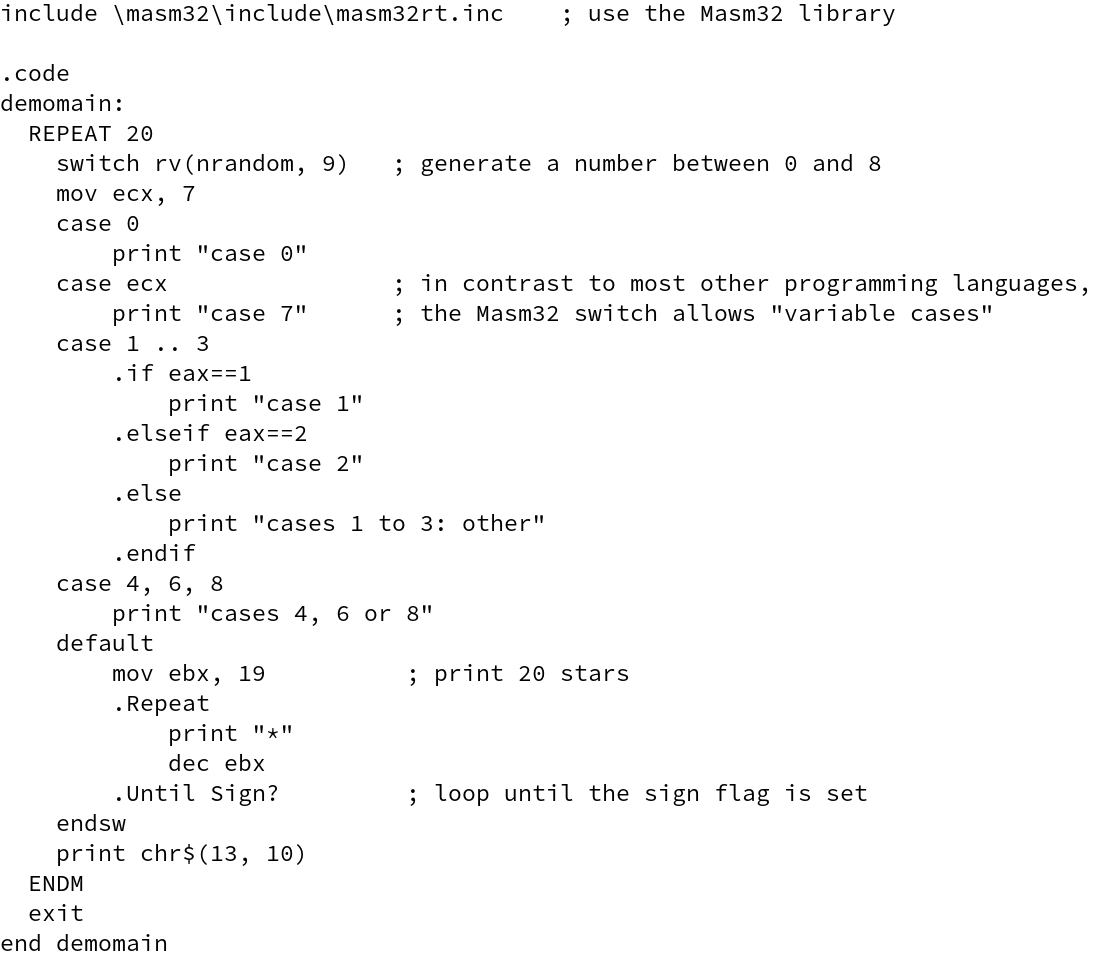
\includegraphics[width=0.6\linewidth]{masm.png}
		\caption{MASM code, Wikipedia ``Assembly Language"}
	\end{figure}
\end{frame}

\begin{frame}{Why?}
	\begin{itemize}
		\item Assemblers (and linkers) optimize by default

		\item Familiar constructs are really
		\bhref{https://www.nasm.us/doc/nasmdoc4.html}{macros} or
		``\bhref{https://www.nasm.us/doc/nasmdoc6.html}{assembler
		directives}"

		\begin{itemize}
			\item \texttt{global \_start} is the user-level
			directive macro of the primitive directive
			\texttt{[global \_start]}

			\item \texttt{section .text} is a convoluted macro for
			\texttt{[section .text]}

			\item Labels are really just memory addresses

			\item ``\texttt{.bss}" just defines memory addresses
			which are writable, and ``\texttt{.text}"
			executable\footnote{see also: self-modifying code}
		\end{itemize}

	\end{itemize}

	No, when compared with languages like C, Lisp, or Scratch, assembly is
	nowhere near high-level.
\end{frame}

\begin{frame}{Why?}
	Assembly cannot be mapped one-to-one with machine code

	\begin{figure}
		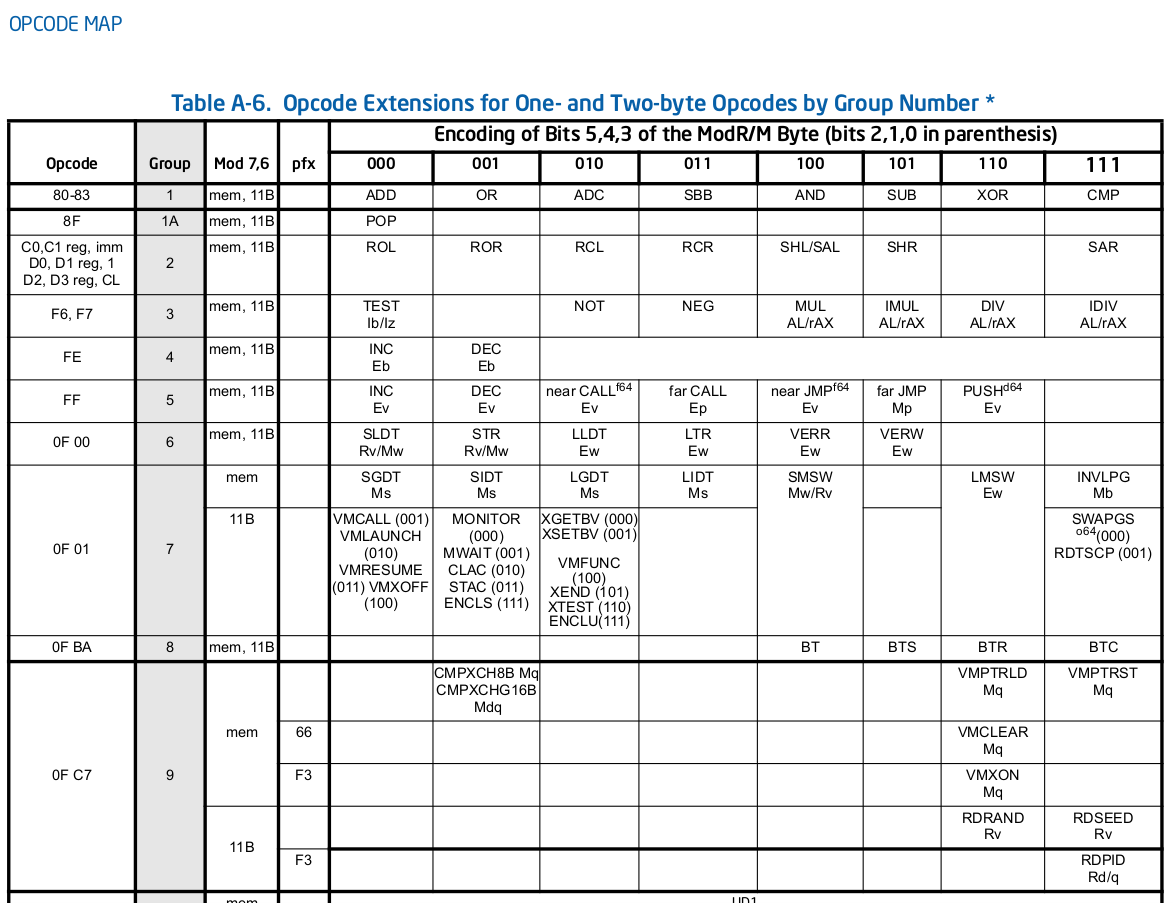
\includegraphics[width=0.65\linewidth]{opcode-table.png}
		\caption{Intel SDM Vol 2D page A-18}
	\end{figure}
\end{frame}

\begin{frame}{Why?}
	\setlength{\parskip}{1em}

	\bhref{https://github.com/xoreaxeaxeax/sandsifter}{github.com/xoreaxeaxeax/sandsifter}

	Tool for finding undocumented x86 instructions. (Also used to find bugs
	in CPU hardware or hypervisors.)

	\textit{On an Intel i5-8250U running Xen 4.8.5-7 through a PVH DomU VM:
	\textbf{89,919 undocumented instructions}.}

	Very few tools allow you to easily execute machine code directly from
	their binary representations.
\end{frame}

\section{To-Do}

\begin{frame}{To-Do}
	What's there left to do?

	\begin{enumerate}
		\item Fix inconsistent endianness and support for writing
		big-endian executables.

		\item Support \texttt{.data} segments

		\begin{enumerate}
		\item Support for specification of arbitrary segments

		\item Work around kernel randomization (position-independent
		executables)
		\end{enumerate}
	\end{enumerate}

	Items 2.1 and 2.2 are required for execution in OpenBSD.
\end{frame}

\section{Tools}

\begin{frame}{Tools}
	\begin{itemize}
		\item \texttt{readelf(1)}

		\begin{enumerate}
			\item \texttt{-eW} (\texttt{--headers --wide})

			\item \texttt{-a} (\texttt{--all})
		\end{enumerate}

		\item \texttt{objdump(1)}

		\begin{enumerate}
			\item \texttt{-d} (\texttt{--disassemble})

			\item \texttt{-D} (\texttt{--disassemble-all})

			\item \texttt{-DFsxwz -M intel}
			(\texttt{--disassemble-all --file-offsets
			--full-contents --all-headers --wide
			--disassemble-zeroes -M intel})
		\end{enumerate}

		\item \texttt{xxd(1)}

		\begin{enumerate}
			\item \texttt{-b} (\texttt{-bits})
		\end{enumerate}

		\item \texttt{strings(1)}
	\end{itemize}
\end{frame}

\section{Resources}

\begin{frame}{Resources}
	\setlength{\parskip}{1em}

	\bhref{https://software.intel.com/en-us/articles/intel-sdm}{Intel 64 and
	IA-32 Architectures Software Developer's Manual} (volume 2 chapter 3,
	appendices A and B) \footnote{specifically the opcode reference, ModR/M,
	and SIB byte tables}

	\bhref{https://developer.amd.com/resources/developer-guides-manuals/}{AMD64
	Architecture Programmer's Manual} (volume 3 chapter 3)

	\bhref{http://refspecs.linuxfoundation.org/elf/gabi41.pdf}{System V
	Application Binary Interface}

	\bhref{http://refspecs.linuxbase.org/elf/x86_64-abi-0.99.pdf}{System V
	ABI AMD64 Architecture Processor Supplement}

	\texttt{elf(5)} (online manuals:
	\bhref{https://man.openbsd.org/man5/elf.5}{1},
	\bhref{http://man7.org/linux/man-pages/man5/elf.5.html}{2})

	\bhref{https://www.muppetlabs.com/~breadbox/software/tiny/teensy.html}{A
	Whirlwind Tutorial on Creating Teensy ELF Executables for Linux}

	Black Hat 2017
	``\bhref{https://www.youtube.com/watch?v=KrksBdWcZgQ}{Breaking the x86
	Instruction Set}" (author of sandsifter)
\end{frame}

\end{document}
